% @Author: AnthonyKenny98
% @Date:   2019-10-30 22:08:06
% @Last Modified by:   AnthonyKenny98
% @Last Modified time: 2020-02-20 01:21:25

% Define Document Class
\documentclass[
    11pt,           % Font Size
    letterpaper,    % Page Size
    draft,          % Draft Mode - error checking and no image rendering
    oneside         % Single Sided
]{report}           % Report Mode
 
% Import custom commands
\RequirePackage{../support/thesis}
\RequirePackage{../newmaster/master}

%%%%%%%%%%%%%%%%%%%%%%%%%%%%%%%%%%%%%%%%%%%%%%%%%%%%%%%%%%

% DEFINE HEADER & FOOTER: (Name and Page Number)
\pagestyle{fancy}
\fancyhf{}
\rhead{Anthony JW Kenny}
\cfoot{\thepage}

% DEFINE COVER PAGE
\title{\textsc{\masterThesisTitle} \\ 
    \bigskip
    \small{A senior design project submitted in partial fulfillment of the requirements for the degree of Bachelor of Science at Harvard University} \\
\author{Anthony JW Kenny \\
        \small{S.B. Candidate in Electrical Engineering} \\ \\
        Faculty Advisor: Vijay Janapa Reddi \\ \\
        Harvard University School of Engineering and Applied Sciences \\
        \small{Cambridge, MA}}
\masterDateAndVersion}


\begin{document}

% Cover Page
\maketitle

% PREFACE
\pagenumbering{roman}
\addcontentsline{toc}{chapter}{Preface}

    % ABSTRACT
    \addcontentsline{toc}{section}{Abstract}
    % @Author: AnthonyKenny98
% @Date:   2019-10-30 22:35:34
% @Last Modified by:   AnthonyKenny98
% @Last Modified time: 2019-10-31 10:45:30

\abstract{This thesis aims to design RISC-V computer architecture that supports the fast execution of motion planning algorithms for drone applications. First, the computation of sampling-based motion planning algorithms commonly used in autonomous drones (such as \ac{RRT}, \ac{RRT*}, \ac{PRM}) will be profiled on an unmodified RISC-V processor. From this profiling, common bottlenecks and hotspots in execution will be identified. Based on these results, this project will extend the RISC-V \ac{ISA} and design a modified processor to support the extensions.}
% 78 words ^
    \clearpage

    % TABLE OF CONTENTS
    \tableofcontents
    \clearpage

    % ACRONYMNS
    \section*{List of Acronyms}
    \addcontentsline{toc}{section}{List of Acronyms}
    \input{\acronymsName}

    % FIGURES
    \listoffigures

    % TABLES
    \listoftables

% CHAPTERS

% Chapter 1
\chapter{Introduction}
    \pagenumbering{arabic}                      % Change Page numbering to arabic
    % @Author: AnthonyKenny98
% @Date:   2020-02-20 00:00:23
% @Last Modified by:   AnthonyKenny98
% @Last Modified time: 2020-02-23 14:27:13



\section{Problem Summary}
    % @Author: AnthonyKenny98
% @Date:   2020-02-23 12:45:54
% @Last Modified by:   AnthonyKenny98
% @Last Modified time: 2020-02-23 14:25:32

\subsection{Background}
    \todo[inline]{TODO: Summarize the following points: \\ 
        1) Need for faster execution of motion planning in drones \\
        2) Strategy of specialized hardware \\
        3) RISC-V ISA and its potentials including extendibility \\
    }

    \subsubsection*{Robotics}
        For well over 2000 years, the concept of robotics, albeit not always with such a term, has fascinated humans. As early as the first century A.D., the Greek mathematician and engineer, Heron of Alexandria, described more than 100 different machines and automata in \textit{Pneumatica} and \textit{Automata}\cite{Alexandrinus}. In 1898, Nikola Tesla demonstrated the first radio-controlled vessel. Since then, the world has seen widespread application of robotics in manufacturing, mining, transport, exploration, and weaponry. For the last few decades, robots have operated in controlled, largely unchanging environments (e.g.\ an assembly line) where their environment and movements are largely known \textit{a priori}.
        \newline
        However, in recent years a new generation of autonomous robots has been developed for a wide range of real-world, complex applications. The increasing trend the use of autonomous robots is shown in Figure \ref{fig:useOfAutonomousRobots}. These new robots, unlike those traditional ones described above, are required to adapt to the changing environment in which they operate. As such, they must perform motion planning in real time.

        % @Author: AnthonyKenny98
% @Date:   2020-02-23 12:12:56
% @Last Modified by:   AnthonyKenny98
% @Last Modified time: 2020-02-23 13:56:51

\begin{figure}%[H]
\begin{center}
\missingfigure[figwidth=\linewidth]{Some sort of line/bar graph showing the increasing use of Autonomous robots over time. Need to find}
% 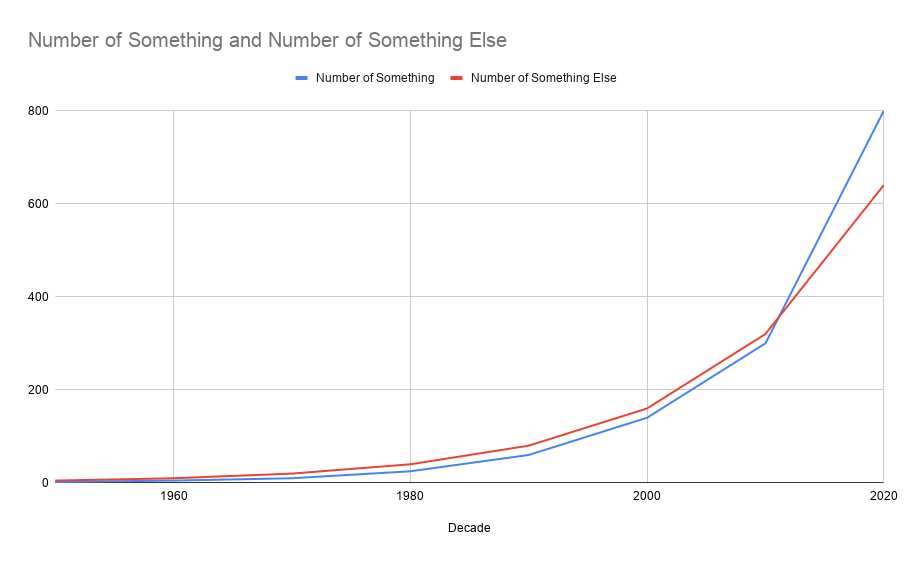
\includegraphics[width=0.8\linewidth]{img/sampleLineGraph.png}
\caption{The use of Autonomous Robots over time}
\label{fig:useOfAutonomousRobots}
\end{center}
\end{figure}

    \subsubsection*{Motion Planning}
        \todo[inline]{TODO: More of an introduction to motion planning.}
        
        Motion Planning refers to the problem of determining how a robot moves through a space to acheive a goal. Chapter \ref{chap:MotionPlanningInSoftware} provides a detailed explanation of motion planning and of \ac{RRT}, a commonly used motion planning algorithm.
        \newline
        On the algorithmic level, motion planning has been extensively studied and many solutions exist. However, current algorithms running on regular \ac{CPU}s are too slow to execute in real time for robots operating in complex environments. Simply solving this problem with more raw computing power, using energy hungry \ac{GPU}s may have merit in tethered robots. On the other hand, untethered applications, such as autonomous drones, where limiting power consumption is a primary concern, this strategy is infeasible.
        
    \subsection*{Hardware Acceleration}
        Specialized hardware designed to perform specific functions can yield significantly higher performance than software running on general purpose processors, and lower power consumption than \ac{GPU}s.
        \todo[inline]{More detail here. Reference prior work}

    \subsubsection{RISC-V}
        \todo[inline]{TODO: Introduction to RISC-V and its merits in this problem}


\subsection{Problem Definition}

    \subsubsection*{Problem Statement}
    \todo[inline]{Revise problem statement}
    Current processors cannot compute motion planning algorithms quickly enough for robots to operate in high complexity environments. Autonomous drones are a specific case of robots requiring real-time motion planning in complex environments. The state-of-the-art strategy of using a Graphics Processing Unit (GPU) to accelerate the execution of these algorithms requires too much power to be cost-effective or feasible for drones to sustain flight for useful periods of time.

    \subsubsection*{End User}
    \todo[inline]{TODO: End User}
    
\section{Prior Work}
    % @Author: AnthonyKenny98
% @Date:   2020-02-23 14:26:30
% @Last Modified by:   AnthonyKenny98
% @Last Modified time: 2020-04-05 08:02:21

\subsection{Hardware Acceleration}
    \Gls{hardware acceleration} refers to the strategy of using computer hardware specifically designed to execute a function more efficiently than can be achieved by software running on a general purpose \gls{CPU}.
    Specialized hardware designed to perform specific functions can yield significantly higher performance than software running on general purpose processors, and lower power consumption than \gls{GPU}s.

    \subsubsection*{Computer Implementation Hierarchy}
        To briefly frame the space in which this thesis operates, consider the typical computer implementation hierarchy, demonstrated in Figure \ref{fig:computerHierarchy}. \textbf{User level applications}, such as Google Chrome, Microsoft Word, and Apple's iTunes, sit at the top of the abstraction hierarchy. These applications are implemented in \textbf{High-Mid Level Languages}, such as C/C++, Python, Java, etc. These programming languages have their own hierarchy, but for the purpose of this thesis, it is sufficient to understand that these programming languages are then compiled into \textbf{Assembly Language}. Assembly language closely follows the execution of instructions on the \textbf{processor}, and is defined by an \textbf{\gls{ISA}}. An \gls{ISA} can be thought of as the contract between software programmers and processor engineers, agreeing what instructions the processor is able to implement. This assembly code is finally loaded into the processor's instruction memory and executed. 
        % @Author: AnthonyKenny98
% @Date:   2020-02-29 23:52:30
% @Last Modified by:   AnthonyKenny98
% @Last Modified time: 2020-04-10 12:37:43
\begin{figure}[H]
\begin{center}
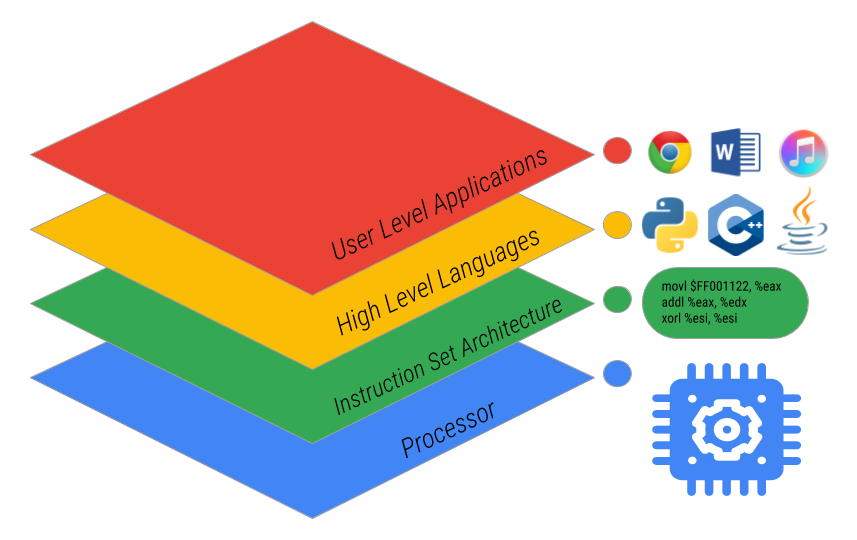
\includegraphics[width=\linewidth]{chapters/chapter1/img/computerHierarchy.png}
\mycaption{Simple Visualization of Computer Implementation Hierarchy}{}
\label{fig:computerHierarchy}
\end{center}
\end{figure}
        As will be outlined in Section \ref{section:projectOverview}, this thesis operates extensively on the lower two levels of this hierarchy, extending an existing \gls{ISA} and building hardware at the processor level that supports these extensions.

    \subsubsection*{Acceleration of Motion Planning}
        Accelerating motion planning with hardware is a fairly well studied problem. \\
        \textit{A Motion Planning Processor on Reconfigurable Hardware} \cite{Atay2006} studied the performance benefits of using \gls{FPGA}-based motion planning hardware as either a motion planning processor, co-processor, or collision detection chip. It targeted the feasibility checks of motion planning (largely collision detection) and found their solution could build a roadmap using the \gls{PRM} algorithm up to 25 times faster than a Pentium-4 3Ghz CPU could. \\
        In \textit{A Programmable Architecture for Robot Motion Planning Acceleration} \cite{Murray}, Murray et al. built on the work of the aformentioned paper, to accelerate several aspects of motion planning in an efficent manner. \\
        \textit{FPGA based Combinatorial Architecture for Parallelizing RRT} \cite{Malik2015} studies the possibility of building architecture to allow multiple \gls{RRT}s to work simultaneously to uniformly explore a map. Taking advantage of hardware parallelism allows systems such as this to compute more information per clock cycle. \\
        Finally, in the paper \textit{Robot Motion Planning on a Chip} \cite{Murrayb}, Murray et al. describe a method for contructing robot-specific hardware for motion planning, based on the method of constructing collision detection circuits for \gls{PRM} that are completely parallelised, such that edge collision computation performance is independent of the number of edges in the graph. With this method, they could compute motion plans for a 6-degree-of-freedom robot more than 3 orders of magnitude faster than previous methods.

    \subsection{RISC-V}
    \subsubsection{Extending RISC-V}
    RISC-V is designed cleverly in a modular way, with a set of base instruction sets and a set of standard extensions. As a result, processors can be designed to only implement the instruction groups it requires, saving time, space and power on instructions that won't be used. In addition, another goal of RISC-V is to provide a basis for more specialized instruction-set extensions or more customized accelerators. This is described in the most recent \textit{RISC-V Instruction Set Manual} \cite{Waterman2019}. This is a powerful feature, as it does not break any software compatability, but allows for designers to easily follow the steps outlined in Figure \ref{fig:extendingRISCV}. From a \gls{hardware acceleration} point of view, this is particularly useful as it allows the designer to directly invoke whatever functional unit or accelerator they implement from assembly code.
    % @Author: AnthonyKenny98
% @Date:   2020-03-01 10:28:34
% @Last Modified by:   AnthonyKenny98
% @Last Modified time: 2020-03-01 10:32:45
\begin{figure}[H]
\begin{center}
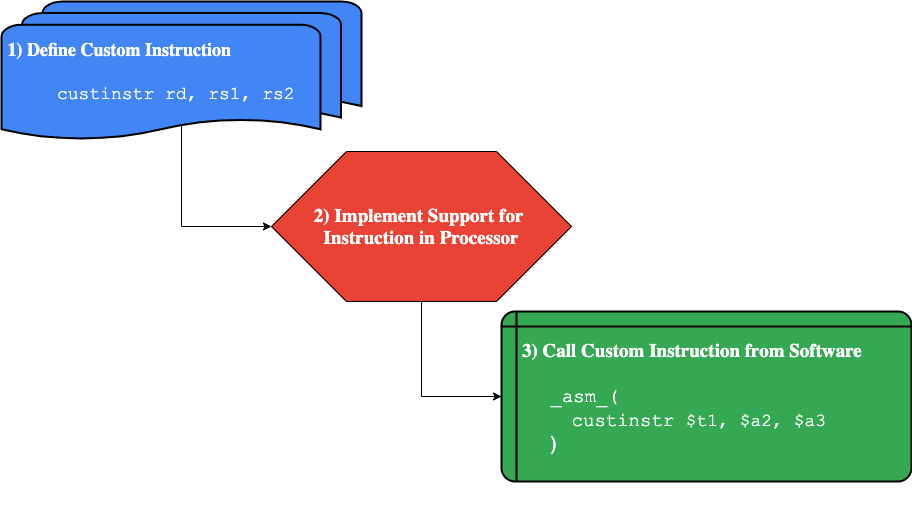
\includegraphics[width=0.9\linewidth]{chapters/chapter1/img/extendingRISCV.png}
\caption{Typical Process of Adding Non-Standard Extension to RISC-V ISA}
\label{fig:extendingRISCV}
\end{center}
\end{figure}

    \subsubsection{Accelerating RISC-V Processors}
    Having only been released in 2011, RISC-V is still a relatively unexplored opportunity for non-education applications. However, it shows promise in the commercial space, with Alibaba recently developing the Xuantie, a 16-core, 2.5GHz processor, currently the fastest RISC-V processor. Recently there has been promising research into accelerating computationally complex applications, particularly in edge-computing, with RISC-V architecture. \\
    \textit{Towards Deep Learning using TensorFlow Lite on RISC-V}, a paper co-written by the faculty advisor of this thesis, V.J. Reddi, presented the software infrastructure for optimizing the execution of neural network calculations by extending the RISC-V ISA and adding processor support for such extensions. A small number of instruction extensions achieved coverage over a wide variety of speech and vision application deep neural networks. Reddi et al. were able to achieve an 8 times speedup over a baseline implementation when using the extended instruction set.
    \textit{GAP-8: A RISC-V SoC for AI at the Edge of the IoT} proposed a programmable RISC-V computing engine with 8-core and convolutional neural network accelerator for power efficient, battery operated, IoT edge-device computing with order-of-magnitude performance improvements with greater energy efficiency. \\



\section{Project Overview}
    % @Author: AnthonyKenny98
% @Date:   2020-02-23 14:27:21
% @Last Modified by:   AnthonyKenny98
% @Last Modified time: 2020-02-23 14:28:10

\subsection{Proposed Solution}
    \todo[inline]{Proposed Solution}


\subsection{Project Specifications}
    \todo[inline]{Project Specifications}

\subsection{Project Structure}
    \todo[inline]{Project Structure/Timeline}



\newpage

    \lhead{Chapter \thechapter}                 % Include Chapter name on subsequent headers


% Chapter 2
\chapter{Background Information}


% Chapter 3
\chapter{RRT}

% % TECHNICAL SPECIFICATIONS
% % @Author: AnthonyKenny98
% @Date:   2019-10-31 10:05:27
% @Last Modified by:   AnthonyKenny98
% @Last Modified time: 2019-10-31 10:47:45


\section{Overall System Specifications}
Let the overall system be defined as 2 part: the Processor Module and the Compiler/Assembler Module. \\
The following subsections detail the technical specifications of the overall system. System specifications based on comparison with benchmarks will be compared against the same programs running on an unmodified, off-the-shelf RISC-V processor synthesized on the same \ac{FPGA}.
\subsection{Speed}
\subsubsection{Quantitative Description}
This project must deliver a system that, given a program that implements, in C, an algorithm often used in autonomous drone motion planning, executes said algorithm an order of magnitude faster than a generic RISC-V processor.

\subsubsection{Justification}
This project aims to achieve a speedup of at least one order of magnitude (10 times) when compared to benchmark performance, in the execution of pure motion planning algorithm programs.
The justification for an order of magnitude speedup comes from similar projects that accelerated motion planning algorithms, acheiving speedups from between 1 and 3 orders of magnitude. These indclude approaches using external hardware accelerators\cite{Murraya}, reprogrammable hardware and parallelization on FPGAs\cite{Murray}\cite{Atay2006}\cite{Malik2015}, and chip redesigns\cite{Murrayb}\cite{Zhi}.

\subsubsection{Measurement}
There will be two broad stages of measurement for this metric. First, in simulation, the Vivado Design Suite\cite{Vivado} will allow the execution of a given compiled program to be timed on a simulated processor that is defined in an \ac{HDL}. Secondly, in synthesis, a to-be-determined tool will allow for me to time the execution of the same program, now on a processor physically synthesized on an FPGA. 

\subsection{Power Consumption}
\subsubsection{Quantitative Description}
This project must deliver a system that has comparable power consumption as an unmodified RISC-V processor operating on the same FPGA. Comparable will be defined as within a tolerance range of 10\%.
\subsubsection{Justification}
Power is defined as energy dissipated over time.\cite{AmericanElectricianHandbook} As such, when considering the application of this system in autonomous drones, we want to minimize the amount electrical energy committed to the computation of paths. Since the primary goal of this thesis is to reduce the execution time, it can aim to keep power use comparable between the benchmark system and the new system. If power remains roughly constant, but the time taken to execute a program is reduced 10 times, we should see a proportional improvement in energy efficiency.
\subsubsection{Measurement}
The Vivado Design Suite\cite{Vivado} will allow for simulated power consumption estimates, but the important measurement will be comparing the new processor to the unmodified processor on the FPGA, running the same program. I am still to determine how exactly to measure this, but the parameters for testing are known and shown above.


\section{Recompiler \& Assembler Specifications}
The first subcomponent of the system is the Compiler \& Assembler Module. It has two specifications, Correctness and Optimality. 
\subsection{Correctness}
\subsubsection{Quantitative Description}
This project must deliver a Compiler \& Assembler Module that, given a program defined in C, can compile and assemble this program into machine code, in a manner that follows the chosen ISA correctly. 
\subsubsection{Justification}
When announcing the IBM System/360 in 1964, IBM said the following: "Instruction Set Architecture is the structure of a computer that a machine language programmer must understand to write a correct program for that machine."\cite{IBM1964} That is, it is a contract between the compiler and the hardware, so that the compiler can write machine code that will work for a given computer processor. In this way, for a given ISA (whether RISC-V, or the extened RISC-V this project will design), the Compiler \& Assembler Module must adhere to that ISA to compile instruction sets that will execute correctly on the processor.
\subsubsection{Measurement}
Testing for correct compiling under the original RISC-V ISA is relatively simple. Does the Generic Compiler (which shouldn't be altered by this project) produce correct RISC-V Assembly. Then, the Recompiler module will operate on those RISC-V assembly instructions to produce a recompiled assembly instruction set that follows the project's extended RISC-V ISA. The Assembler will then assemble this into machine code that can be directly loaded into the processor's Instruction Memory. Testing for this required extensive and complete unit tests to be written during this project.

\subsection{Optimality}
\subsubsection{Quantitative Description}
This project must deliver a Compiler \& Assembler Module that, given certain extended instructions that this project defines, recompiles all regular RISC-V assembly code that is suitable for recompilation. 
\subsubsection{Justification}
The RISC-V \ac{ISA} is an ISA that supports user-level ISA extensions and specialized variants\cite{Isa2012}, which may allow the number of instructions per program to be reduced through clever redesign of a processor and new instructions. However, to reap the full performance rewards of these extensions, a compiler must use the new instructions whenever it is able.
\subsubsection{Measurement}
This will be challenging to measure. I plan to write extensive unit tests that will determine manually the optimal recomplication from RISC-V to extended RISC-V assembly, and then compare that to the output of the recompiler module. There will also be tests to check that these substitutions are occuring in larger, more complicated programs.

\section{Processor Specifications}
The second subcomponent of the system is the Processor Unit. It has two specifications, RISC-V Compliance and Syntheizability.

\subsection{RISC-V Compliance} \label{subsection:riscvCompliance}
\subsubsection{Quantitative Description}
The project must deliver a processor that is RISC-V Compliant, meaning that it can support any correctly compiled RISC-V Assembly Code.
\subsubsection{Justification}
A processor must be such that it supports the execution of all instructions defined in the \ac{ISA} for which it was designed. So too must this project's finished processor be able to correctly support any correctly compiled RISC-V assembly code. This may range from simple programs compiled into either the original or extended RISC-V \ac{ISA}, to complete operating systems, whether for drone applications or a generic linux distribution, for example. 
\subsubsection{Measurement}
The RISC-V organisation has provided a Github Repo for testing a processor for RISC-V compliance.\cite{Compliance} Once it passes this, this processor should be able to run any program or OS compiled into RISC-V assembly.

\subsection{Synthesizable}
\subsubsection{Quantitative Description}
The project must deliver a processor defined in an \ac{HDL} that is synthesizable on an FPGA for the project to be useful for drone developers. While this project will use and test with the Diligent Zync-7000 \ac{SoC}\cite{Zync}, the design should be synthesizable on most Zync boards.
\subsubsection{Justification}
Many papers that have worked in the area of accelerating motion planning algorithms for robot applications have delivered a finished product of a processor/accelerator design implemented in an \ac{HDL} for synthesis on an FPGA.\cite{Murray}\cite{Atay2006}\cite{Malik2015} This FPGA can then be used to control the robot or share computational load with a co-processor.
\subsubsection{Measurement}
Measurement for this specification is relatively simple. Once the processor is designed in an \ac{HDL}, it can be synthesized onto an FPGA using the Vivado Design Suite, given the design is synthesizable (although this is not always simple to achieve). If it is not synthesizable, the design suite will throw and error.
Finally, while the design should be correct and RISC-V compliant by the tests performed in section \ref{subsection:riscvCompliance}, to be safe, these compliance tests along with any other unit tests designed during this thesis will then be run on the \ac{FPGA} processor.

% \section{Analysis}
% The design process has, quite necessarily, begun with significant anaylsis of the RRT algorithm. This section will first describe RRT, and then explain my analysis of the algorithm.

% \subsection{RRT}
% % @Author: AnthonyKenny98
% @Date:   2019-11-02 18:44:43
% @Last Modified by:   AnthonyKenny98
% @Last Modified time: 2019-11-02 19:53:49

\SetArgSty{textnormal}

\ac{RRT} is an algorithm designed to efficiently search, and thus plan a path through, a high-complexity environment by randomly sampling points and building a tree. The algorithm randomly samples points, draws an edge from the nearest currently existing node in the tree, to grow the tree in the space. It is inherently biased to grow towards large unsearched areas of the problem. RRT was developed by S. LaVelle \cite{LaValle1998} and J. Kuffner \cite{LaValle2001}. It is used in autonomous robotic motion planning problems such as autonomous drones, the focus of this thesis. \\

The RRT Algorithm with Collision Detection can be seen in Algorthim 1.

\begin{algorithm}[H]
\SetAlgoLined
\textbf{Inputs:} Space $S$ with obstacles \\ 
\textbf{Output:} Collision free graph $G$ with $K$ nodes \& edges \\
    $G$.init()\;
    \For{$k = 1$ to $K$}{
        \While { !\text{pointCollision}($node_{new}$) } {
            $q_{rand} \leftarrow $ getRandomNode(); \\
            $q_{near} \leftarrow $ findNearestNode(); \\
            $q_{new} \leftarrow $ stepFromTo(); \\
        }
        $e_{new} \leftarrow $ newEdge($q_{near}, q_{new}$) \\
        \eIf{\text{!edgeCollision($e_{new}$)}} {
            $G$.addNode($q_{new}$); \\
            $G$.addEdge($e_{new}$);
        }{
            $k = k-1$;
        }
    }
 \caption{Rapidly-exploring Random Tree with Collision Detection}
\end{algorithm}

% \subsection{RRT Profiling}
% % @Author: AnthonyKenny98
% @Date:   2019-11-02 19:23:52
% @Last Modified by:   AnthonyKenny98
% @Last Modified time: 2019-11-03 00:28:50

To restate, the aim of this thesis is to design a computer processor with reduced execution time of motion planning algorithms, such as \ac{RRT}. As such, it is important to understand the elements of the algorithm that have the highest percentage of CPU execution time. To determine this, it was necessary to implement my own, naive but typical, \ac{RRT} in C. This program could then be compiled and analysed using a software performance profiling tool. With this, I could design experiments to determine the critical RRT functions (those occupying a majority of CPU time) and see how this varies given different paramaters.

\subsubsection{Implementation of Algorithm}
The first step was to source a simple, naive implementation of RRT in C that could be analysed. The two options were to either find an existing, public implementation or to develop my own. Many implementations I found online\cite{RoboJackets2019}\cite{Planning2019}\cite{Sourishg2017}\cite{Vss2sn2019} were unsuitable for my purposes, as they had extraneous \ac{GUI}s, reliance on external \ac{API}s, and other features that distorted analysis of algorithmic hotspots. This made them largely useless for my performance analysis. I needed a clean, minimal implementation of RRT so that I could easily identify the percentage of CPU time each function took up.  \\ 

As such, I implemented my own version. It can be found \href{https://github.com/AnthonyKenny98/Thesis/tree/master/my_rrt}{here}. It follows the Algorithm defined above closely. I took care to be able to parametrize factors such as Number of Nodes, Number of Obstacles, Obstacle Size, State Space Size, and Epsilon (acceptable distance between two nodes). For monitoring correctness, I build in an optional \ac{GUI} that shows the tree, starting node, and obstacles. Figure \ref{table:rrtGui} demonstrates the \ac{GUI} and the \ac{RRT} implementation.

\begin{figure}[H]
\begin{center}
\begin{tabular}{c  c}
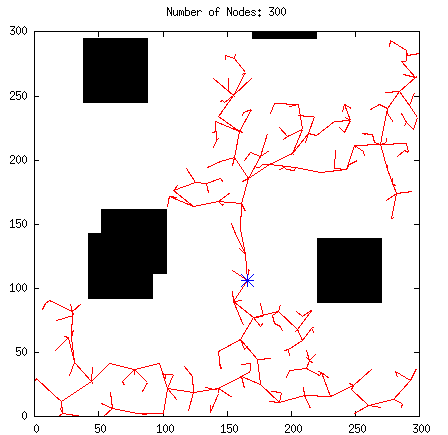
\includegraphics[width=0.5\linewidth]{../master/rrt/img/sampleRRT1.png} & 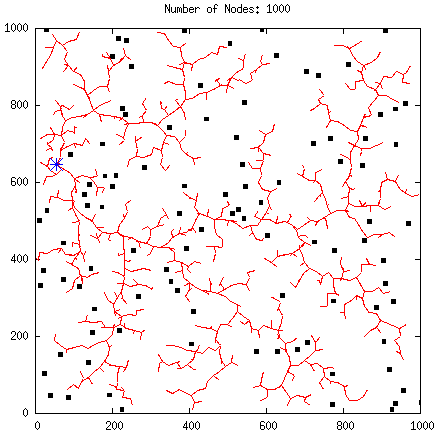
\includegraphics[width=0.5\linewidth]{../master/rrt/img/sampleRRT2.png} \\
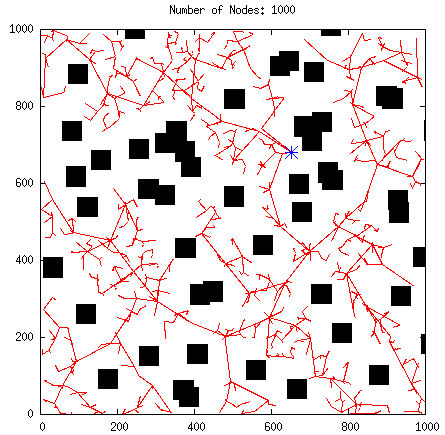
\includegraphics[width=0.5\linewidth]{../master/rrt/img/sampleRRT3.png} & 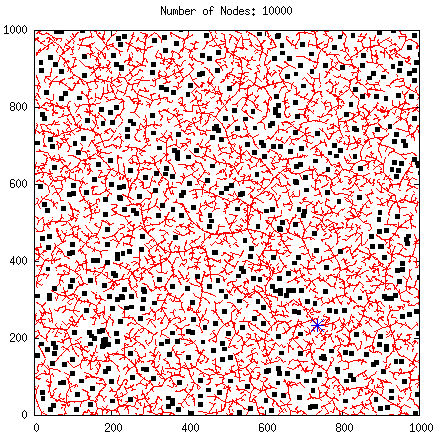
\includegraphics[width=0.5\linewidth]{../master/rrt/img/sampleRRT4.png}
\end{tabular}
\caption{RRT Implementation shown by \ac{GUI}}
\label{table:rrtGui}
\end{center}
\end{figure}

\subsubsection{Top Down Analysis}{}

The idea of top-down analysis is a practical method to quickly identify true bottlenecks in out-of-order processors, explained well in the paper by A. Yasin\cite{Yasin2014}. It was influenced by a basic approach that examines the functions that take the highest percentage of CPU time, and drills down to examine their sub-routines. This functionality is provided by software by Intel, called VTune Amplifier. \\

VTune Amplifier performance profiler is an application for software performance analysis. It provides functionality to examine hotspots for CPU execution time through a top down analysis, shown below in Figure \ref{fig:topdown}. As can be seen from the figure, the top down analysis tool shows the percentage of CPU time taken up by each function. I used this tool to profile the algorithm's performance as I changed certain parameters.

\begin{figure}[H]
\begin{center}
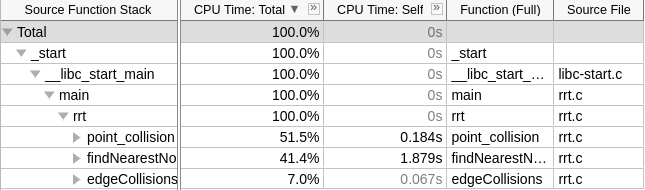
\includegraphics[width=0.8\linewidth]{../master/rrt/img/topDownAnalysis.png}
\caption{Top Down Analysis Functionality provided by VTune Amplifier}
\label{fig:topdown}
\end{center}
\end{figure}


\subsubsection{Experimental Design}

As stated above, I parametrized my implementation to be able to vary state space, number of nodes, number of obstacles, obstacle size, and  Epsilon. When considering the application of autonomous drones, the two most important factors are number of nodes and number of obstacles. Number of nodes is important for any implementation of RRT, as this is a determining factor of execution speed. A higher number of nodes will also yield shorter paths/higher probability of finding a path to a goal. Number of obstacles is important for autonomous drones, as the obstacles they face in their operating environments (complex natural environments) are often irregularly shaped. As such, these obstacles must often be discretized into a number of smaller obstacles. This is unlike applications such as robotic arms, where the size of (often regularly shaped) obstacles is more important. Given this, I ran a series of tests, varying number of nodes and number of obstacles, to determine the relative use of CPU time for each sub-routine in my RRT implementation.

\newpage

\subsubsection{Results}
The left side of Figure \ref{table:rrtPerformance} shows \% of CPU use for a given number of nodes, while the right side shows the same but for a given number of obstacles. the results below show that the three main sub-functions within the \ac{RRT} implementation are \texttt{edgeCollision()}, \texttt{pointCollision()}, and \texttt{findNearestNode()}. The importance of this is discussed in the design section.
\begin{figure}[H]
\begin{center}
\begin{tabular}{c | c}
Given \# of Nodes                                           & Given \# of Obstacles \\  
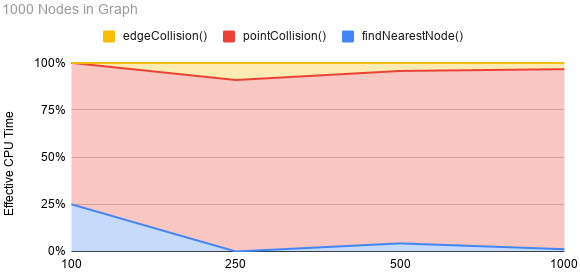
\includegraphics[width=0.45\linewidth]{../master/rrt/img/performance/nodes/1000nodes.png} & 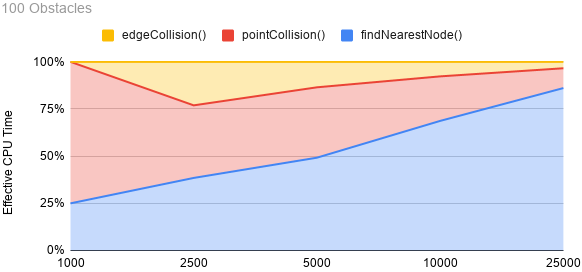
\includegraphics[width=0.45\linewidth]{../master/rrt/img/performance/obs/100obs.png} \\
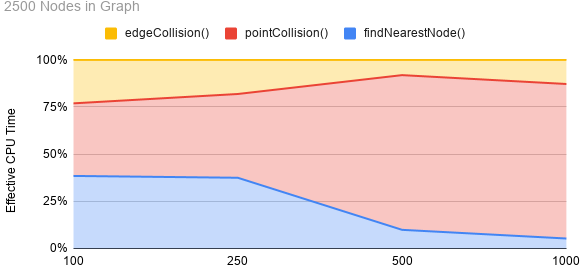
\includegraphics[width=0.45\linewidth]{../master/rrt/img/performance/nodes/2500nodes.png} & 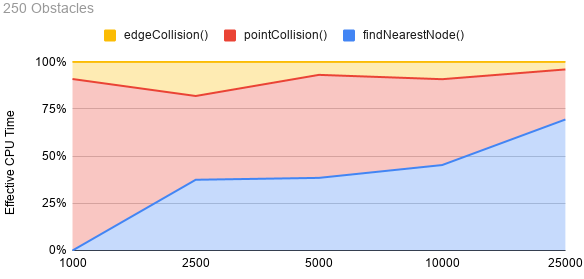
\includegraphics[width=0.45\linewidth]{../master/rrt/img/performance/obs/250obs.png} \\
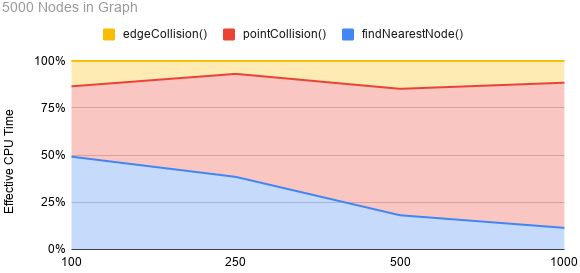
\includegraphics[width=0.45\linewidth]{../master/rrt/img/performance/nodes/5000nodes.png} & 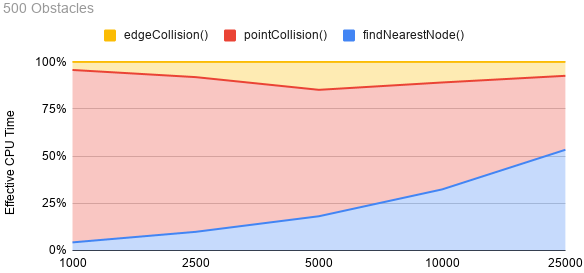
\includegraphics[width=0.45\linewidth]{../master/rrt/img/performance/obs/500obs.png} \\
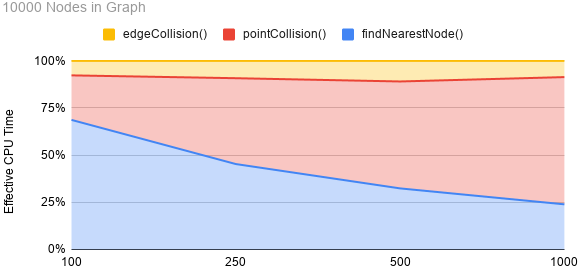
\includegraphics[width=0.45\linewidth]{../master/rrt/img/performance/nodes/10000nodes.png} & 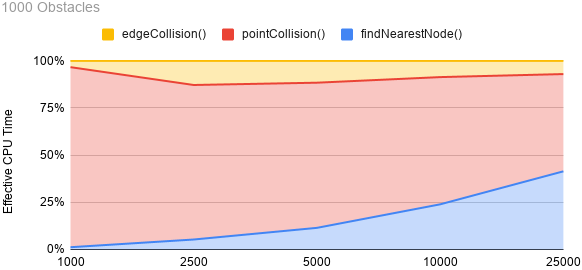
\includegraphics[width=0.45\linewidth]{../master/rrt/img/performance/obs/1000obs.png} \\
\end{tabular}
\caption{\% of CPU Time per Function}
\label{table:rrtPerformance}
\end{center}
\end{figure}




% \section{Design}

% \subsection{System Diagram}
% The overall system can be defined as two subcomponents: a Compiler \& Assembler Module, and a modified RISC-V Processor.

% \begin{center}
% 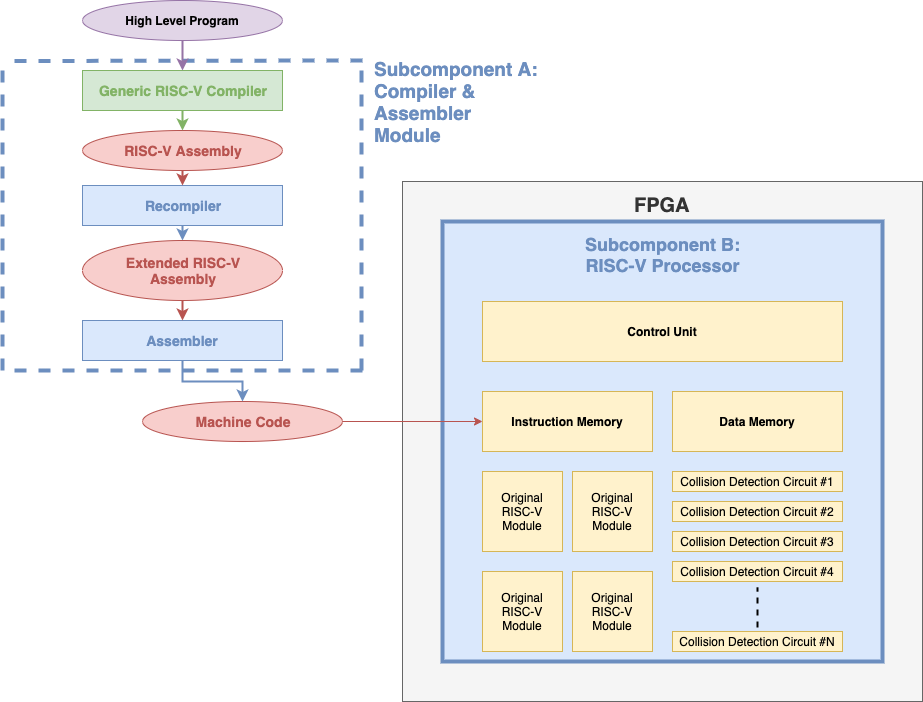
\includegraphics[width=\linewidth]{../newmaster/img/systemDiagramHorizontal.png}
% \end{center}

% \subsection{Subcomponent B Design}
% As can be seen in the \ac{RRT} profiling results shown in Figure \ref{table:rrtPerformance}, \texttt{pointCollision()} occupies the majority of CPU execution time. Looking at the graphs on the left, where for each graph the number of nodes remain constant, it can be seen that for a given number $K$ of nodes in a graph, the percentage of CPU time occupied by \texttt{pointCollision()} increases. When considering the application of RRT to autonomous drones, it is important to note that improving performance as obstacles increase (and the space becomes more complex) is crucial. As such, it makes the most sense to target the execution of \texttt{pointCollision()} on the processor. \\

% S. Murray et al., in their paper \"Robot Motion Planning on a Chip\" describes a method for reducing the execution time of collision detection within the context of the \ac{PRM} algorithm.\cite{Murrayb} They introduced the concept of a \ac{CDC}. They implement a series of $N$ collision detection circuits on the processor, where $N$ is the maximum number of nodes in the graph, to simultaneously compute which nodes collide with obstacles in the state space. While their approach centered on discretizing the state space into a series of "depth pixels", I believe that the necessary calculations to perform the \texttt{pointCollision()} function can be converted into boolean logic and built into a set of $N$ \ac{CDC}s in my modified RISC-V processor. \\

% I will be implementing the entire processor in a \ac{HDL}, most likely Verilog, and then using Xilinx to simulate the processor and synthesize onto an FPGA. Due to setbacks in the approach I will be taking to actually synthesize the processor, the board has only just been ordered, and will arrive soon for me to start this process.

% \subsection{Subcomponent A Design}
% I've placed the Subcomponent A Design section beneath Subcomponent B in this document because it logically follows that the design of Subcomponent A will rely very much on the ultimate design of Subcomponent B. The design of the extended instructions for the RISC-V ISA will depend on how the \ac{CDC}s interact with the processor, and how best to feed these calculations from the control module to the \ac{CDC}s in the processor. As such, much of this is currently unknown and will depend on how the project develops. I do know that I will rely on the RISC-V GNU toolchain (available on GitHub) to compile C code. From there, I will need to convert assembled code from basic RISC-V to my extended RISC-V ISA.


% \section{Logistics}
% \subsection{Project Timeline}

% \begin{center}
% \begin{tabular}{ |m{0.7\linewidth}|m{0.3\linewidth}|}
%     \hline
%     \textbf{Project Milestone}                                      & \textbf{Completion Date} \\
%     \hline
%     Checkpoint 2: Design Documentation                              & 3 November 2019 \\
%     \hline
%     Synthesize RISC-V Processor on FPGA                         & 17 November 2019\\
%     \hline
%     Checkpoint 3: Mid Year Presentation                             & 3 December 2019 \\
%     \hline
%     Synthesize with successful \ac{CDC}s                           & 15 December 2020 \\
%     \hline
%     Implement RISC-V Extensions and Compiler Module                                & 29 December 2020 \\
%     \hline
%     Complete First Round Analysis                                   & 12 January 2020 \\
%     \hline
%     Checkpoint 4: Poster Session and Peer Reviews               & 9 February 2020 \\
%     \hline
%     Second Design Iteration and Analysis                            & 23 January 2020 \\
%     \hline
%     Checkpoint 5: Report Draft                                      & 28 February 2020 \\
%     \hline
%     More Analysis                            & 8 March 2020 \\
%     \hline
%     Finalize Presentation and Report                            & 22 March 2020 \\
%     \hline
%     Final Oral Presentation                                         & 24 March 2020 \\
%     \hline
%     Final Written Report                                            & 3 April 2020 \\
%     \hline
%     Final Poster                                                    & 6 May 2020 \\
%     \hline
    
% \end{tabular}
% \end{center}

% \subsection{Budget}
% \begin{center}
% \begin{tabular}{ |c|c|c|}
%     \hline
%     \textbf{Item}           & \textbf{Link}                                                     & \textbf{Cost} \\
%     \hline
%     Zynq Board              & \href{https://www.xilinx.com/products/boards-and-kits/1-elhabt.html}{https://www.xilinx.com/products/boards-and-kits/1-elhabt.html}     & \$495 \\
%     \hline
% \end{tabular}
% \end{center}

\bibliography{\bibliographyName}
\bibliographystyle{ieeetr}

\begin{appendices}

\chapter{Appendix 1}

\end{appendices}

\clearpage



\end{document}  
